\documentclass [handout]{beamer}
\usetheme{metropolis}
%\mode<presentation>
%\mode<handouts>

\AtBeginSection[]{
  \begin{frame}
  \vfill
  \centering
    \begin{beamercolorbox}[sep=8pt,center,shadow=true,rounded=true]{title}
    \usebeamerfont{title}\insertsectionhead\par%
    \end{beamercolorbox}
  \vfill
  \end{frame}
}

\title[Discrete Math]{A Short Course in Discrtete Mathematics for the Computer Science Undergraduate}
\author{Dale Fletter}
\institute{UC Davis, ECS20, Summer Session 2}
\date{}
\usepackage{graphicx} % support the \includegraphics command and options
\usepackage {graphics}
\graphicspath{ {../../Outline-tex/illustrations/} }






\begin{document}
\begin{frame}
\titlepage
\end{frame}

\section{Propositional Logic}
\begin{frame}{Proposition}
A proposition is a declarative sentence which is true or false, but not both. Also called a statement. In symbolic logic we use single lowercase letters beginning with p to represent propositions. These are called \textit{propositional variables}.
\end{frame}

\begin{frame}{Compound Proposition}
A \textbf{compound proposition} is a proposition formed from atomic propositions with logical connectives or logical operators. Also called a logical or Boolean expression. An atomic propositions is one that is not a compound propositions.
\end{frame}

\begin{frame}{Negation}
Let $p$ be a proposition. The \textit{negation of p}, denoted by $\lnot p$ (also denoted by $\overline{p}$, is the statement 
\textit{"It is not the case that $p$."}\\
The proposition $\lnot p$ is read "not $p$". The truth value of the negation of $p$,  $\lnot p$, is the opposite of the truth value of $p$.
\end{frame}

\begin{frame}{Conjunction}
Let $p$ and $q$ be propositions. The \textit{conjunction} of $p$ and $q$, denoted by $ p \land q$, is the proposition \textit{p and q}. The conjunction $p \land q$ is true when both $p$ and $q$ are true and is false otherwise.
\end{frame}

\begin{frame}{Disjunction}
Let $p$ and $q$ be propositIons. The disjunction of $p$ and $q$, denoted by $p \lor q$, is the proposition \textit{p or q}. The disjunction $p \lor q$ is false when both $p$ and $q$ are false and true otherwise.
\end{frame}

\begin{frame}{Exclusive OR}
Let p and q b propsition. The \textit{exclusive or} of $p$ and $q$, denoted by $p \oplus q$, is the proposition that is true when exactly one of $p$ and $q$ is true and is false otherwise.
\end{frame}

\begin{frame}
\begin{table}[htbp]
   \centering
   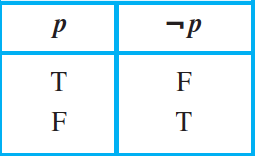
\includegraphics [width=1.5in]{Table-1-1-1-Negation}
   \caption{The Truth Table for the Negation of a Proposition}
   \label{table:negation}
   \end{table}
\end{frame}

\begin{frame}
\begin{table}[htbp]
   \centering
   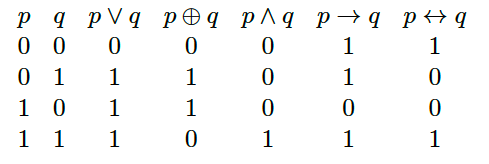
\includegraphics [width=4in]{Table-1-1-9-TableOfBitwiseLogic}
   \caption{Bitwise Logic}
   \label{table:bitwiselogic}
\end{table}
\end{frame}

\begin{frame}
\begin{table}[htbp]
   \centering
   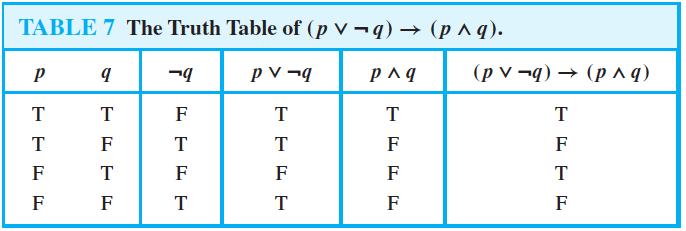
\includegraphics [width=4in]{Table-1-1-7-ExamTruthTable}
   \caption{Evaluation of a Compound Proposition}
   \label{table:EvalCompoundProp}
\end{table}
\end{frame}

\begin{frame}{Precedence of Elementary Logical Operators}
\begin{table}[htbp]
   \centering
   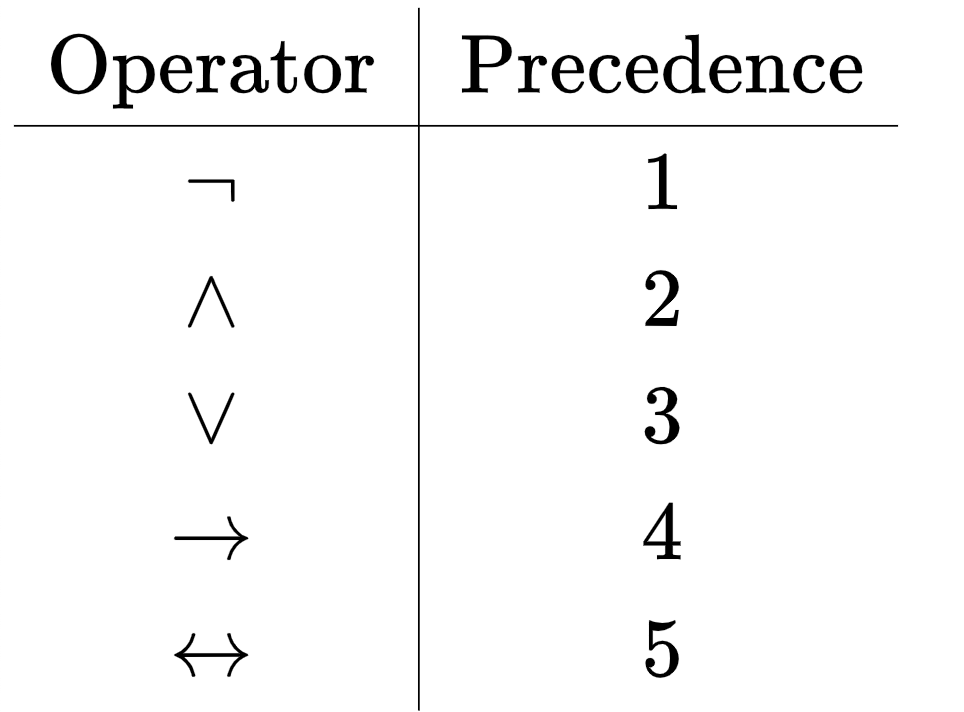
\includegraphics [width=1.5in]{PrecedenceOfLogicalOperators}
   \caption{Precedence of Logical Operators}
   \label{table:precedenceOfLogicalOperators}
\end{table}
\end{frame}

\begin{frame}{Bitstring  Operations}
A bit is a binary digit, typically a zero or a one. A bit string is a sequence of zero or more bits. The length of this string is the number of bits in the string. Given two bit strings of the same length we define bitwise operations:
\begin{enumerate}
\item bitwise OR, 
\item bitwise AND, 
\item bitwise XOR.
\end{enumerate}
\end{frame}


\section{Material Implication}
\begin{frame}{Implication/Conditional}
Let $p$ and $q$ be propositions. The conditional statement $p \rightarrow  q$ is the proposition "if p then q".  The conditional statement $p \rightarrow q$ is false when $p$ is true and $q$ is false, and true otherwise. In the conditional statement  $p \rightarrow q$, $p$ is called the \textbf{hypothesis} (or \textbf{antecedent} or \textbf{premise}) and $q$ is called the \textbf{conclusion} or \textbf{consequent}.  
\end{frame}

\begin{frame}{Inverse, Converse, Contrapositive}
Given a conditional statement $p \rightarrow q$, 
\begin{enumerate}
\item its \textbf{inverse} is the statement $q \rightarrow p$, 
\item its \textbf{converse} is $\lnot p \rightarrow \lnot p$ and 
\item its \textbf{contrapositive} is the statement $\lnot q \rightarrow \lnot p $
\end{enumerate}
\end{frame}

\begin{frame}{Biconditional}
Let $p$ and $q$ be propositions. The \textit{biconditional statement} $p \leftrightarrow q$ is the proposition "$p$ if and only if $q$." The biconditional statement $p \leftrightarrow q$ is true when $p$ and $q$ have the same truth values, an d is false otherwise. Biconditional statements are also called \textit{bi-implicatons}. We can also read this as "p is logically equivalent to q". 
\end{frame}

\begin{frame}{Tautology and Contradiction}
A compound proposition that is always true , no matter what the truth value of the poisitons that occur in it, is called a \textit{tautology}. A compound proposition that is always false is called a \textit{contradiction}. A compound proposition that is neither a tautology nor a contradiction is called a \textit{contingency}.
\end{frame}

\begin{frame}{Logical Equivalence}
The compound proposition $p$ and $q$ are called \textit{logically equivalent} if $p \leftrightarrow q$ is  tautology. The notation $p \equiv q$ denotes that $p$ and $q$ are logically equivalent.
\end{frame}

\begin{frame}
\begin{table}[htbp]
  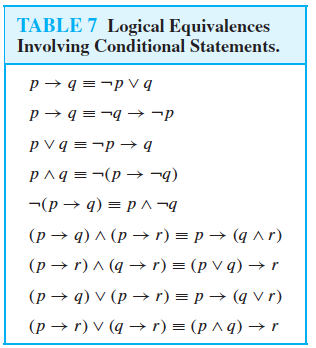
\includegraphics [width=2in]{Table-1-6-7-LogicalEquivalencesInvolvingConditionalStatements}
  \caption{Logical Equivalences Involving Conditional Statements}
  \label{table:logicalequivalencesinvolvingconditionalstatements}
  \end{table}
\end{frame}

\begin{frame}
\begin{table}[htbp]
  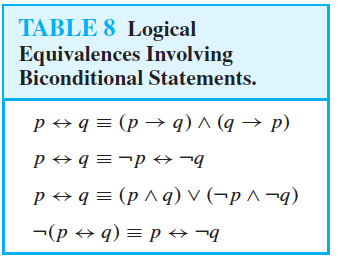
\includegraphics [width=3in]{Table-1-6-8-LogicalEquivalencesInvolvingBiconditonalStatements}
  \caption{Logical Equivalences Involving Bi-Conditional Statements}
  \label{table:LogicalEquivalenceInvolvingBiconditionalStatements}
  \end{table}
\end{frame}

\begin{frame}{Rule of Substitution}
Whenever two compound propositions are equivalent, one may be substituted for the other with no impact on the truth value.
\end{frame}

\begin{frame}{An Algebra of Propositional Logic}
\begin{table}[htbp]
  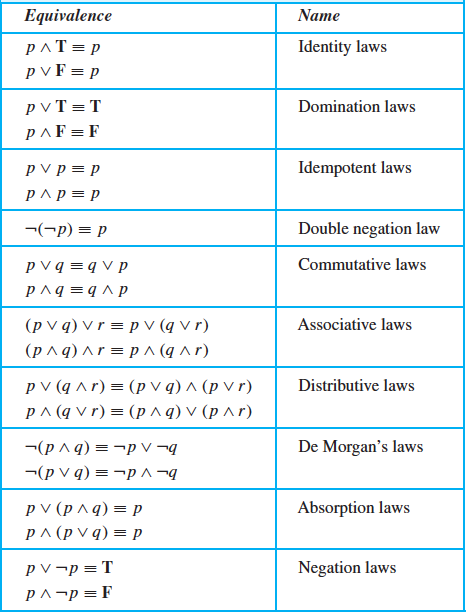
\includegraphics [width=1.8in]{Table-1-3-6-LogicalEquivalences}
  \caption{Logical Equivalences}
  \label{table:LogicalEquivalence}
  \end{table}
\end{frame}

\begin{frame}{Consistency}
A group of propositions are said to be \textit{consistent} if and only if there is some assignment of truth values to the atomic propositions that make all of the given propositions true in at least one case.
NOTE: system specifications that are not consistent can never be satisfied.
\end{frame}

\begin{frame}
\begin {enumerate}
\item Abbott is a gunslinger.
\item Bob is a gunslinger or Charleen is a pugalist. 
\item Charleen is a pugalist and Davida is a bartender.
\end{enumerate}
Extract the atomic propositions...
\end{frame}

\begin{frame}
\begin{enumerate}
\item p: Abbott is a gunslinger
\item q: Bob is a gunslinger
\item r: Charleen is a pugalist.
\item s: Davida is a bartender.
\end{enumerate}
Now restate original sentences symbolically...
\end{frame}

\begin{frame}
\begin{enumerate}
\item $p$
\item $q \lor r$
\item $r \land s$
\end{enumerate}
Now build truth table and search for at least one row where all the original assertions can be true.
\end{frame}

\begin{frame}
\footnotesize
\begin{table}
\begin{tabular}{l | c | c | c | c | c }
$p$ & $q$ &$ $r & $s$ & $q \lor r$ & $r \land s$ \\
\hline \hline
T & T & T & T & T & T \\ 
T & T & T & F & T & F \\ 
T & T & F & T & T & F \\ 
T & T & F & F & T & F \\ 
T & F & T & T & T & T \\ 
T & F & T & F & T & F \\ 
T & F & F & T & F & F \\ 
T & F & F & F & F & F \\ 
F & T & T & T & T & T \\ 
F & T & T & F & T & F \\ 
F & T & F & T & T & F \\ 
F & T & F & F & T & F \\ 
F & F & T & T & T & T \\ 
F & F & T & F & T & F \\ 
F & F & F & T & F & F \\ 
F & F & F & F & F & F \\ 
\end{tabular}
\caption{Are the propositions consistent?}
\end{table}
\normalfont
\end{frame}

\begin{frame}
The last problem can be solved through deduction.
$p$ must be true.
$r$ and $s$ must be true.
$q$ can be either true or false.

The two combinations are TTTT and TFTT.
\end{frame}

\begin{frame}{Paradox}
Some declarative statements defy taking a truth value. For example, ``This statement is false'' cannot be assigned either true or false. It it is false, then the statement must be true. But if it is true, then the statement must be false. Such a statement is called a \textbf{paradox}.
\end{frame}

\begin{frame}{A Smullyan Logic Puzzle}
Knights always tell the truth.\\
Knaves always lie.\\
No other possibilities.

p: person who answered door is a knight\\
q: other person in house is a knight
\begin{table}
\begin{tabular}{l | c   }
$p$ & $q$   \\
\hline \hline
T & T   \\ 
T & F   \\ 
F & T   \\ 
F & F   \\ 

\end{tabular}
\caption{Who lives in the house?}
\end{table}
\end{frame}

\begin{frame}{Another Smullyan Puzzle}
A census taker comes to the door where two people live. The person who answers says, ``We are both knaves.'' What do you conclude?

Translate into propositions. Two people, each can either be a knave or a knight. 
p: A is a knight
q: B is a knight
\end{frame}


\section{Predicate Logic}
\begin{frame}
Propositional logic is sometimes called ``zeroeth order logic''. There is reasoning that cannot be done with it like, ``Socrates is a man, all men are mortal, therefore Socrates is mortal". The ancient Greeks had worked out a form of reasoning for this kind of challenge but we found a new way in the 19thc and now use a different form which we call  \textit{Predicate Logic}, \textit{Predicate Calculus} or \textit{first order logic}. There are other higher order logics. 
\end{frame}


\begin{frame}{Predicates}
A \textit{predicate} is a function which when applied to an object will evaluate to true when some property is present and false otherwise. We denote the predicate using a capital letter and write the expression using a functional notation. 

We often define a predicate using a notation like, $P: x+1 > 0$.

So the predicate $P$ when applied to the variable $x$ is written $P(x)$ and will take on the value of true or false when the value of $x$ has been fixed (bound).
\end{frame}

\begin{frame}{N-Place Predicates}
Predicates are not limited to one argument but can have any number of arguments, called \textit{n-place predicates}. For example the predicate $S$ could be "...have the same color" and can accept pieces of fruit as objects. Then the expression $S(p,q,r,s,t)$ will be true if the color of each piece of fruit $p,q,r,s,t$ matches the others and false otherwise.

\end{frame}

\begin{frame}{Binding and Scope}
Variables can be bound to values. But we often wish to assert a proposition over a range of values or to claim that there is an object with some property. This process of creating a proposition over some range of objects is called \textit{quantification}. The two fundamental quantifications are the universal and the existential.
\end{frame}

\begin{frame}{Universal Quantification}
Quantification]\index{universal quantification}
The universal quantification of P(x) is the statement 
$$\text{"}P(x) \text{ for all values of }x \text{ in the domain."}$$
The notation $\forall x P(x)$ denotes the universal quantification of $P(x)$. Here $\forall$ is called the universal quantifier. We read $\forall x P(x)$ as "for all x P(x)" or "for every x P(x)". An element for which $P(x)$ is false is called a counterexample of $\forall x P(x)$.
\end{frame}

\begin{frame}{Existential Quantification}
The \textit{existential quantification} of $P(x)$ is the proposition
$$\text{"There exists an element }x \text{ in the domain such that } P(x) \text{ ."}$$
We use the notation $\exists x P(x)$ for the existential quantification of $P(x)$. Here $\exists$ is called the \textbf{existential quantifier}.
The domain must always be specified when a statement $\exists P(x)$ is used. The meaning of $\exists P(x)$ changes when the domain changes. without specifying the domain, the statement $\exists P(x)$ has no meaning. The existential quantifier $\exists P(x)$ is read as, "There is an $x$ such that $P(x)$, "There is at least one $x$ such that $P(x)$", or "For some $x P(x)$".
\end{frame}

\begin{frame}{Uniqueness}
The \textit{uniqueness quantification} of $P(x)$ is the proposition:
$$\text{"There exists exactly one element }x \text{ in the domain such that }P(x)\text{".}$$
We use the notation $\exists !$ for the uniqueness quantification.
\end{frame}

\begin{frame}{Binding and Scope of Variables}
When a variable has been assigned a value, we say the value has been \textbf{bound} to the variable. Any variable that has not yet been bound to a value is said to be \textbf{free}. The \textbf{scope} of the binding is controlled by the use of parentheses or other marks. The value of a variable is also bound by the use of a quantifier and the variable is either within or outside the scope of that quantifier.
\end{frame}

\begin{frame}
 \begin{table}[htbp]
  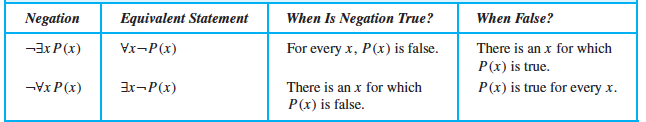
\includegraphics [width=3in]{DeMorgansForQuantifiedExpressions}
  \caption{DeMorgansForQuantifiedExpressions}
  \label{table:DeMorgansForQuantifiedExpressions}
  \end{table}
\end{frame}

\begin{frame}{Restricted Domains}
An abbreviated notation is sometimes used to specify some subset of the domain. For example $\forall x <0 (x^2 >0)$ in the domain of real numbers places the restrictive clause next to the quantifier.
\end{frame}

\begin{frame}{Variable Binding and Scope}
When a variable has been assigned a value, we say the value has been \textbf{bound} to the variable. Any variable that has not yet been bound to a value is said to be \textbf{free}. The \textbf{scope} of the binding is controlled by the use of parentheses or other marks. The value of a variable is also bound by the use of a quantifier and the variable is either within or outside the scope of that quantifier.

Universal quantifiers at the outermost level can be omitted, i.e., free variables are interpreted as universally quantified at the outermost level. Quantifiers can be applied to more than one variable at once (e.g., $\forall x,y$). 
\end{frame}

\begin{frame}{Logical Equivalence of Quantified Expressions}
Statements involving predicates and quantifier are \textit{logically equivalent} if and only if they have trhe same truth value no matter which predicates are substitued into these statements and which domain of discourse is used for the variables in these propositionan functions. We use the notation $S \equiv T$ to indicate that two statements $S$ and $T$ involving predicates and quantifiers are logically equivalent.
\end{frame}

\begin{frame}
    \begin{table}[htbp]
  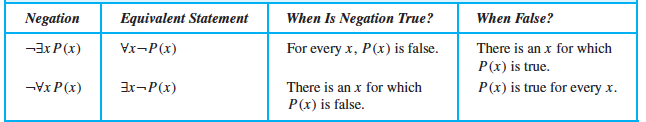
\includegraphics [width=3in]{DeMorgansForQuantifiedExpressions}
  \caption{DeMorgansForQuantifiedExpressions}
  \label{table:DeMorgansForQuantifiedExpressions}
  \end{table}
\end{frame}

\begin{frame}{Quantification of Two Variables}
\begin{table}[htbp]
  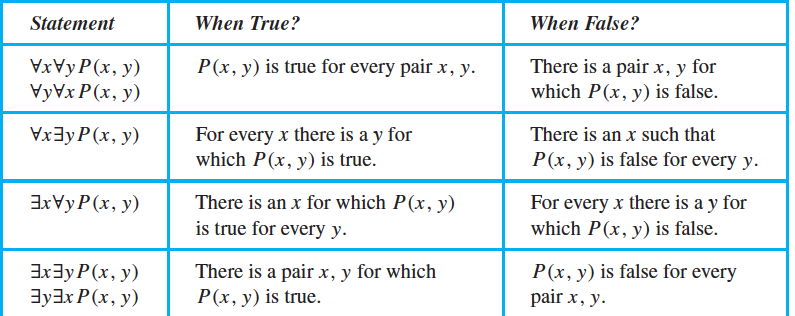
\includegraphics [width=3in]{Table-1-5-1-QuantificationsOfTwoVariables}
  \caption{Quant Of 2 Var}
  \label{table:QuantificationOfTwoVariables}
  \end{table}
\end{frame}

\begin{frame}{The Order of Quantifiers in an Expression}
It is important to note that the order of the quantifiers can make a difference. For example is this statement true or false for the domain of integers? $\forall x \exists y : (x+y=10)$. This is easily proven true with a bit of algebra. But what about $\exists y \forall x : (x+y=100)$. This is false since there is no such integer that will always give 10 when added to any other integer. 
\end{frame}


\begin{frame}{Seeing Nested Quantified Expressions as Loops}
\end{frame}


\begin{frame}
\frametitle{There Is No Largest Prime Number}
\framesubtitle{The proof uses \textit{reductio ad absurdum}.}
\begin{theorem}
There is no largest prime number.
\end{theorem}
\begin{proof}
\begin{enumerate}
\item<1-| alert@1> Suppose $p$ were the largest prime number.
\item<2-> Let $q$ be the product of the first $p$ numbers.
\item<3-> Then $q+1$ is not divisible by any of them.
\item<1-> But $q + 1$ is greater than $1$, thus divisible by some prime
number not in the first $p$ numbers.\qedhere
\end{enumerate}
\end{proof}
\end{frame}








\end{document}